\section{Operator spreading and finite optimality}

The minimal plaquette model is used to test whether the finite-regime logic identified in the curvature analysis reappears in real-time dynamics. We therefore compute the dynamics as a function of the loop coupling $\lambda$ and ask whether operator spreading, correlation persistence, and entanglement organization all remain simultaneously effective in a bounded interval rather than at the strongest available loop term.

Operator spreading is tracked through the out-of-time-ordered echo
\begin{equation}
F(t)
=
\langle W^\dagger(t)V^\dagger W(t)V\rangle,
\end{equation}
with the plotted OTOC metric defined as $1-\mathrm{Re}\,F(t)$. In the numerical sweep we average over three probe configurations: two computational-basis initial states and one $|+\!+\!+\!+\rangle$ state, together with distinct Pauli choices for $(W,V)$. This keeps the finite-optimality claim from depending on a single probe. Long-time correlation persistence is quantified by the late-time average of nearest-neighbor $ZZ$ correlators, while stability is quantified through a one-qubit entanglement factor that is largest at intermediate entropy and suppressed near both product-state and over-scrambled limits.

The resulting dynamical score is
\begin{equation}
S_{\rm dyn}(\lambda)
=
A_{\rm spread}(\lambda)\,
A_{\rm corr}(\lambda)\,
A_{\rm stability}(\lambda).
\end{equation}
Here $A_{\rm spread}$ is the normalized mid-time OTOC amplitude, $A_{\rm corr}$ is the normalized late-time correlation persistence, and $A_{\rm stability}$ is the intermediate-entropy factor extracted from the subsystem entanglement. This definition is intentionally finite-regime in character: it rewards spreading only when it coexists with correlation retention and dynamical stability.

Figure~\ref{fig:fig4_plaquette_dynamics} shows the three regimes clearly. For small $\lambda$, operator spreading remains weak and the OTOC grows only modestly. For an intermediate loop strength $\lambda^\star$, the OTOC develops strongly while long-time correlations remain appreciable and the entanglement remains in the structured intermediate range. For large $\lambda$, operator spreading is still present, but correlation persistence degrades and the combined score drops, indicating overdriven or scrambled dynamics rather than a useful finite EDT regime. For the nominal sweep shown in Fig.~\ref{fig:fig4_plaquette_dynamics}, with $J=0.4$ and $h=0.4$, the maximum occurs at $\lambda^\star = 0.8$, while representative small- and large-coupling points are $\lambda = 0.15$ and $\lambda = 1.25$, respectively.

The finite optimum is not a single-point artifact of the nominal controls. Panel (e) of Fig.~\ref{fig:fig4_plaquette_dynamics} shows the extracted $\lambda^\star$ under variation of the transverse field $h$ for several $J$ values. The optimum shifts with control parameters, as expected for a real dynamical landscape, but it remains interior over a substantial part of the sweep rather than collapsing to $\lambda=0$ or to the largest tested loop strength. This is the key dynamical result of the minimal model: finite EDT behavior appears as a bounded optimum in operator spreading and correlation persistence, not as monotonic improvement with increasing nonlocal control.

\begin{figure*}[t]
\centering
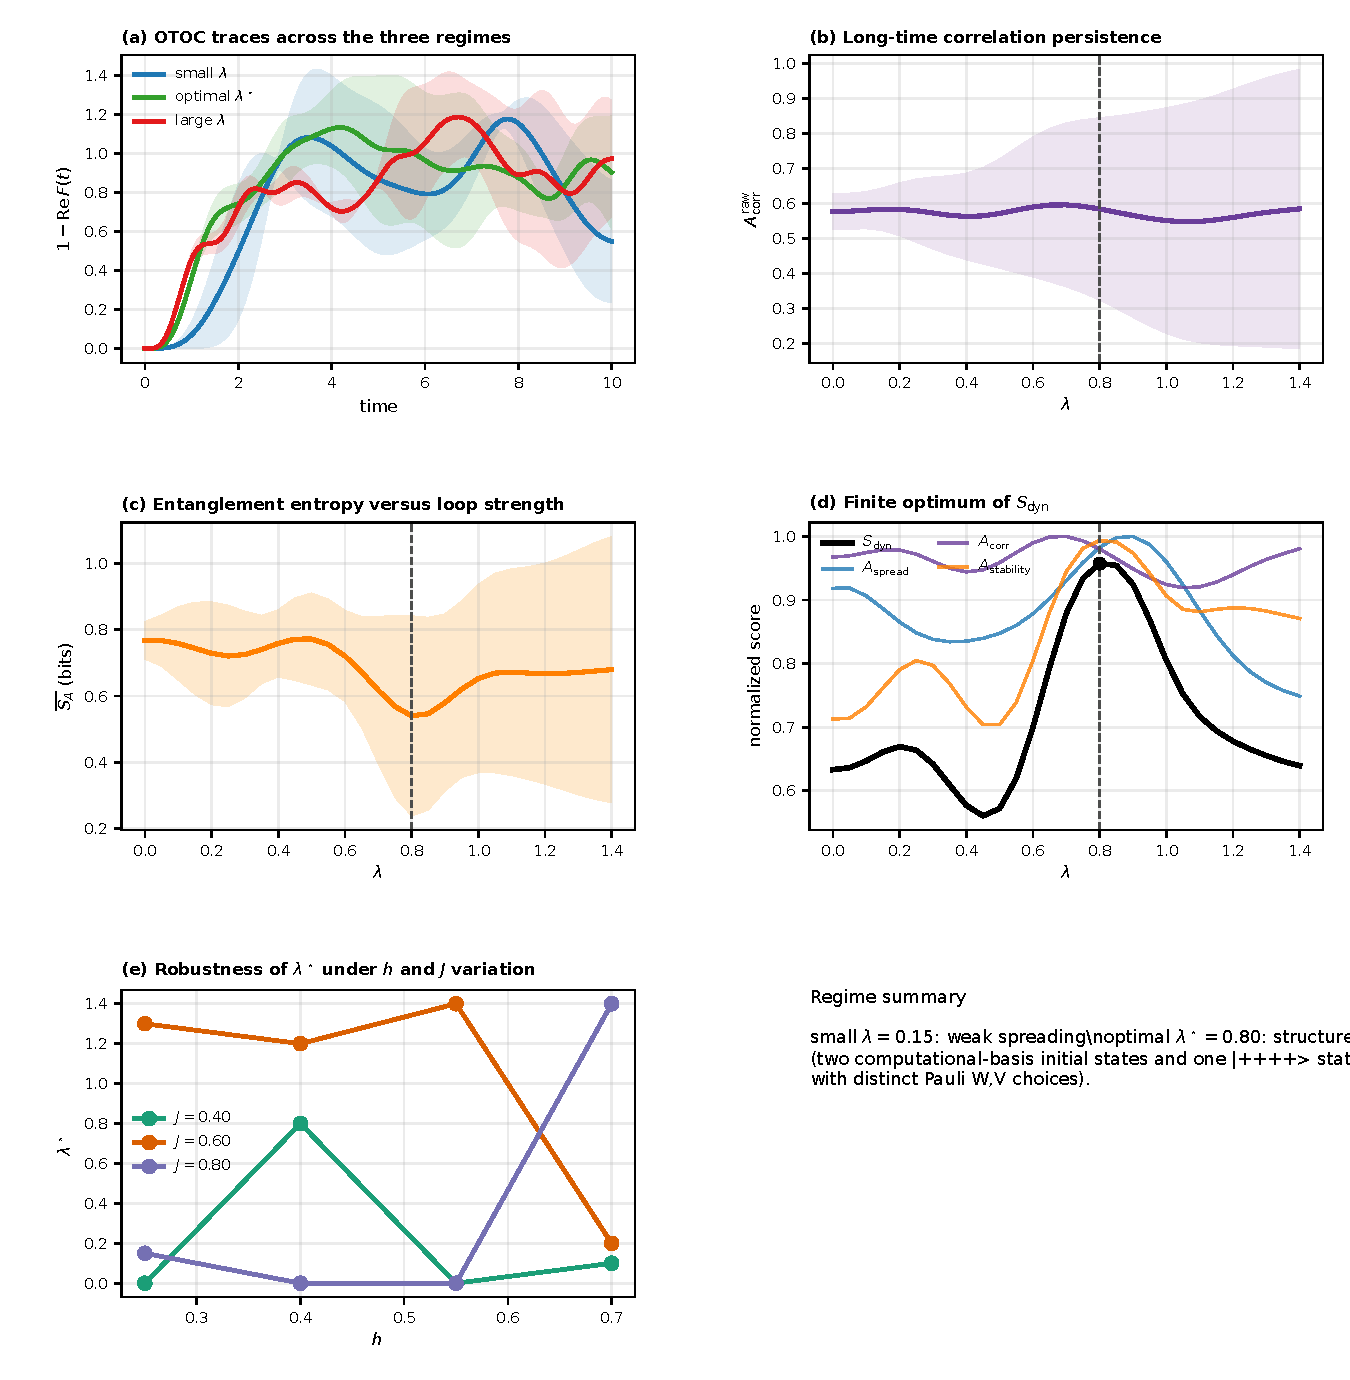
\includegraphics[width=0.96\linewidth]{fig4_plaquette_dynamics.pdf}
\caption{\textbf{Operator spreading and finite optimality in the minimal plaquette model.}
(a) Probe-averaged OTOC traces, plotted as $1-\mathrm{Re}\,F(t)$, for representative small, optimal, and large loop couplings. (b) Late-time nearest-neighbor correlation persistence versus $\lambda$. (c) One-qubit entanglement entropy versus $\lambda$. (d) Composite dynamical score $S_{\rm dyn}=A_{\rm spread}A_{\rm corr}A_{\rm stability}$, showing a finite optimum at intermediate loop strength. (e) Robustness of the optimal loop coupling $\lambda^\star$ under variation of $h$ for several fixed $J$ values. The figure is generated by \texttt{scripts/fig4\_plaquette\_dynamics.py}, and the processed sweep data are written to \texttt{data/processed/plaquette\_lambda\_sweep.csv}.}
\label{fig:fig4_plaquette_dynamics}
\end{figure*}
